\documentclass[10pt]{beamer}

\newcommand{\lectnum}{L05}
\newcommand{\lecttitle}{Introduction to Neural Networks}

\usepackage{amsmath, amssymb, graphicx}
\usepackage[]{algorithm2e}
\usepackage{pdfpages}
\usepackage[british]{babel}

\hypersetup{colorlinks,linkcolor=,urlcolor=blue}
\newenvironment{titledslide}[1]{\begin{frame}\frametitle{#1}}{\end{frame}}

\mode<presentation>{\setbeamercovered{transparent}}

\setbeamertemplate{sidebar right}{}
\setbeamertemplate{footline}{%
\hfill\usebeamertemplate***{navigation symbols}
\hspace{0.4cm}\lectnum: \insertframenumber{}/\inserttotalframenumber \hspace*{0.4cm}}

\author{James Cussens}

\title{COMS30035, Machine learning:\\ \vspace{5pt} \lecttitle}

\institute{School of Computer Science\\University of Bristol}

\begin{document}
%%%%%%%%%%%%%%%%%%%%%%%%%%%%%%%%%%%%%%%%%%%%%%%%%%%%%%%%%%%%%%%%%%%%%%

\begin{frame}
  \titlepage
\end{frame}

%%%%%%%%%%%%%%%%%%%%%%%%%%%%%%%%%%%%%%%%%%%%%%%%%%%%%%%%%%%%%%%%%%%%%%

\begin{document}
%%%%%%%%%%%%%%%%%%%%%%%%%%%%%%%%%%%%%%%%%%%%%%%%%%%%%%%%%%%%%%%%%%%%%%

\begin{frame}
  \titlepage
\end{frame}
%%%%%%%%%%%%%%%%%%%%%%%%%%%%%%%%%%%%%%%%%%%%%%%%%%%%%%%%%%%%%%%%%%%%%%
\begin{titledslide}{Acknowledgement}

  \begin{itemize}
  \item These slides are adapted from ones originally created by
    \href{https://www.dpag.ox.ac.uk/team/rui-ponte-costa}{Rui Ponte
      Costa} and later edited by Edwin Simpson and James Cussens. 
  \end{itemize}
  
\end{titledslide}
%%%%%%%%%%%%%%%%%%%%%%%%%%%%%%%%%%%%%%%%%%%%%%%%%%%%%%%%%%%%%%%%%%%%%%
\begin{frame}[fragile]
  
  \frametitle{Agenda}
  \begin{itemize}
  \item Perceptron
  \item Neural networks (multi-layer perceptron)
    \begin{itemize}
    \item Architecture
    \item The backpropagation algorithm
    \item Gradient descent
    \end{itemize}
  \end{itemize}

\end{frame}
%%%%%%%%%%%%%%%%%%%%%%%%%%%%%%%%%%%%%%%%%%%%%%%%%%%%%%%%%%%%%%%%%%%%%%          





\begin{frame}[fragile]
\frametitle{Perceptron -- a simplified neural network}



\begin{itemize}
	\item It is the very beginning of neural network models in ML! \vspace{3pt}\\
	\item It is directly inspired by how neurons process information: \vspace{3pt}\\	
	\centerline{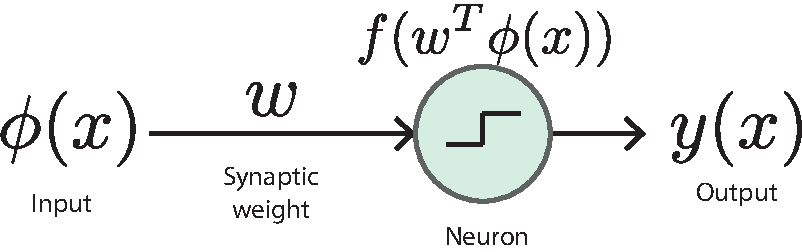
\includegraphics[scale=0.4]{figures/Rosenblatt_neuron.pdf}}
\uncover<2->{	\item It is an example of a linear discriminant model given by $y(\bm{x}) = f(\bm{w}^T\phi(\bm{x}))$\\ 
	with a nonlinear \emph{activation function} $f(a) = \begin{cases}
+1, &a \geq 0 \\
-1, &a < 0
\end{cases} $}
\uncover<3->{
\item Here the target $t = \{+1, -1\}$.
\item And we aim to minimise the following error $ - \mathlarger{\sum_{n=1}^N \bm{w}^T\phi_nt_n }$ \footnote{Intuitively we want to improve our chances of having $t_n = y_n = -1$ or $t_n = y_n = 1$, which will both decrease our error function.}}
\end{itemize}

\end{frame}



\begin{frame}[fragile]
\frametitle{Perceptron -- a simplified neural network}


% \begin{example}
\centerline{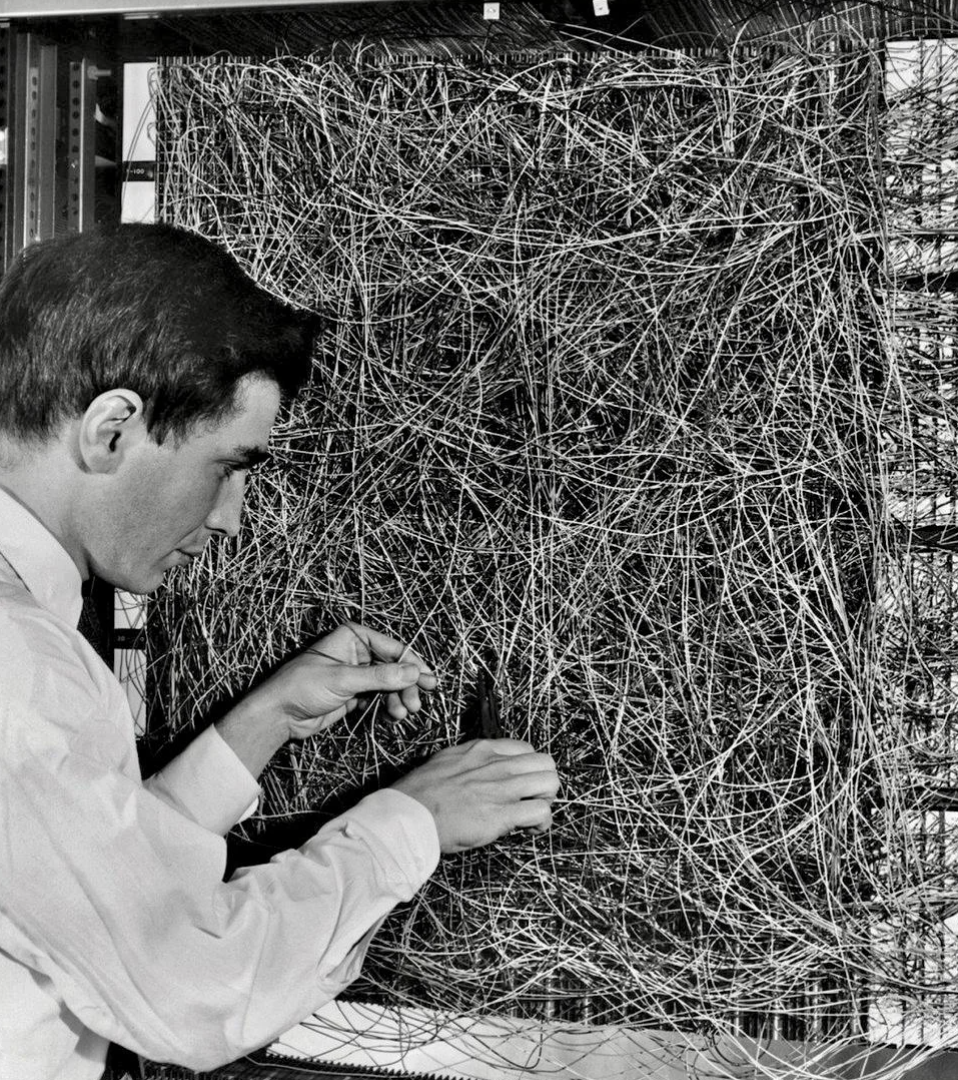
\includegraphics[scale=0.15]{figures/Rosenblatt.png}}
\textbf{\textcolor{red}{The Perceptron of Rosenblatt (1962)}}\\
Perceptrons started the journey to the current \emph{deep learning} revolution!

Frank Rosenblatt used IBM and special-purpose hardware for a parallel implementation of perceptron learning. 

Marvin Minksy, showed that such models could only learn \emph{linearly separable problems}. 

For example, the XOR problem could not be solved by the perceptron model.
% However, this limitation is only true in the case of single layers!
% \end{example}

{\fontsize{6}{6} \selectfont source: Bishop p193.}

\end{frame}

%---------------------
\begin{frame}{XOR problem}
\begin{itemize}
    \item Label $1$: Points $(1,0)$ and $(0,1)$
    \item Label $0$: Points $(0,0)$ and $(1,1)$
\end{itemize}
\centering
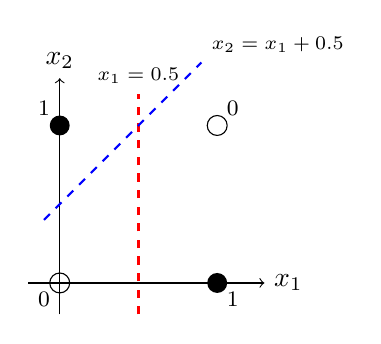
\begin{tikzpicture}[scale=2]
  % axes
  \draw[->] (-0.2,0) -- (1.3,0) node[right] {$x_1$};
  \draw[->] (0,-0.2) -- (0,1.3) node[above] {$x_2$};

  % points: class 0 (circles), class 1 (filled)
  \fill (1,0) circle (1.8pt) node[below right] {\footnotesize 1};
  \fill (0,1) circle (1.8pt) node[above left] {\footnotesize 1};
  \draw (0,0) circle (1.8pt) node[below left] {\footnotesize 0};
  \draw (1,1) circle (1.8pt) node[above right] {\footnotesize 0};

  % candidate separating lines (dashed)
  % Line 1: vertical x1 = 0.5
  \draw[dashed,red,thick] (0.5,-0.2) -- (0.5,1.2)
        node[above,black] {\scriptsize $x_1=0.5$};
  % % Line 2: diagonal x2 = x1
  % \draw[dashed,blue,thick] (-0.1,-0.1) -- (1.2,1.2)
  %       node[above right,black] {\scriptsize $x_2=x_1$};
  % Line 2: diagonal x2 = x1 + 0.5 (passes through (0,0.5))
  \draw[dashed,blue,thick] (-0.1,0.4) -- (0.9,1.4)
        node[above right,black] {\scriptsize $x_2=x_1+0.5$};
\end{tikzpicture}

\medskip
\small \uncover<2->{No single straight line separates the positive and negative points.}

\uncover<3->{This limitation can be solved by a multi-layer perceptron (MLP)}.
% \centering
% \begin{tikzpicture}[scale=2]
%   % axes
%   \draw[->] (-0.2,0) -- (1.3,0) node[right] {$x_1$};
%   \draw[->] (0,-0.2) -- (0,1.3) node[above] {$x_2$};
%   % points: class 0 (circles), class 1 (filled)
%   \fill (1,0) circle (1.8pt) node[below right] {\footnotesize 1};
%   \fill (0,1) circle (1.8pt) node[above left] {\footnotesize 1};
%   \draw (0,0) circle (1.8pt) node[below left] {\footnotesize 0};
%   \draw (1,1) circle (1.8pt) node[above right] {\footnotesize 0};
%   % (Optional) tell students: try any line—one positive and one negative swap sides.
% \end{tikzpicture}
\end{frame}


%
%\begin{frame}[fragile]
%\frametitle{Linear separability}
%
%\begin{example}
%To illustrate We generated data using two  for two classes . The main features are the petal and sepal size, samples below for 2 classes ($K=2$). \\
%	\begin{itemize}
%		\item \textcolor{darkgray}{$C = \{\text{iris setosa, iris versicolor}\}$
%		\item $x = \{ \text{petal size, sepal size} \}$}
%	\end{itemize}
%	
%\centerline{\includegraphics[scale=0.3]{../figures/iris_dataset_2classes.png}}
%\end{example}
%
%\end{frame}
%
%
%\begin{frame}[fragile]
%\frametitle{The Iris dataset}
%
%\begin{example}
%The iris dataset is one of the most popular datasets used in ML. The main features are the petal and sepal size, samples below for 2 classes ($K=2$). \\
%	\begin{itemize}
%		\item \textcolor{darkgray}{$C = \{\text{iris setosa, iris versicolor}\}$
%		\item $x = \{ \text{petal size, sepal size} \}$}
%	\end{itemize}
%	
%\centerline{\includegraphics[scale=0.3]{../figures/iris_dataset_2classes.png}}
%\end{example}
%
%\end{frame}


\begin{frame}[fragile]
\frametitle{Neural networks}

From a single layer perceptron:\\

	\centerline{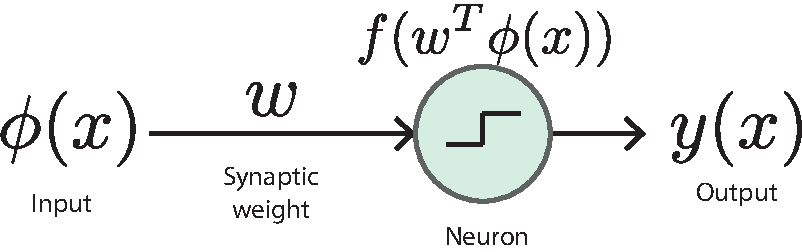
\includegraphics[scale=0.5]{figures/Rosenblatt_neuron.pdf}}
	
%However these and other linear (or near-linear) models have limited expressibility due to the \emph{curse of dimensionality}.

\end{frame}


\begin{frame}[fragile]
\frametitle{Neural networks}

To a Multiple Layer Perceptron (MLP) \footnote{Although, we call it
  perceptron, it typically uses logistic {\color{blue} sigmoid} activation functions
  (continuous nonlinearities), instead of step-wise discontinuous
  nonlinearities. 
  % NB the first and second weight vectors will be
  % different, despite both being denoted by $w$ here.
  }:\vspace{5pt}\\

	\centerline{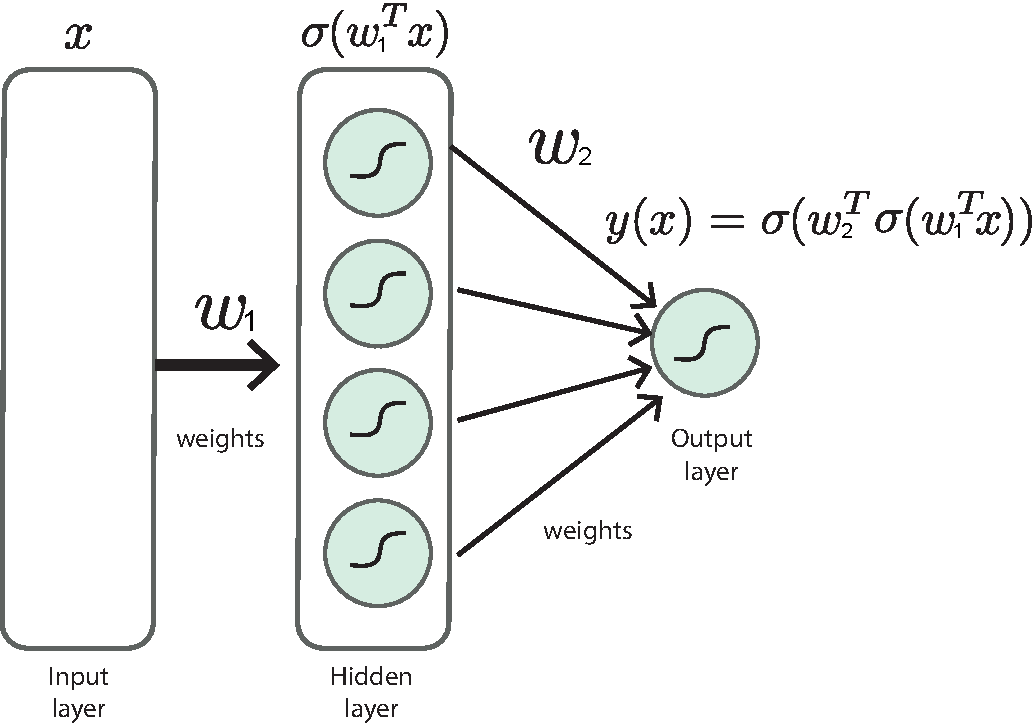
\includegraphics[scale=0.5]{figures/MLP_variant.pdf}}

\end{frame}


\begin{frame}[fragile]
\frametitle{Neural networks}


\begin{itemize}
	\item Neural networks are at heart composite functions of linear-nonlinear functions. 
	\item \textbf{Deep learning}\footnote{If you would like to learn more take our Applied Deep Learning unit in your 4th year.} refers to neural networks (or MLPs) with more than 1 hidden layer\\	
	\item They can be applied in any form of learning, but we will focus on \underline{supervised learning} and classification in particular\\	
\uncover<2->{	\item MLP recipe \footnote{Here we focus on simple feedforward nets but the recipe is the same for any neural network.}:
	\begin{itemize}	
		\item Define architecture (i.e.\ how many hidden layers and neurons) \footnote{Note that this makes them parametric models.}
		\item Define cost function (e.g.\ mean squared error)
		\item Optimise network using backprop:
			\begin{enumerate}	
				\item Forward pass -- calculate activations; generate $y_k$
				\item Calculate error/cost function	
				\item Backward pass -- use backprop to
                                  compute error gradient
                                \item Use gradient to improve parameters 
			\end{enumerate}	
	\end{itemize}}
\end{itemize}

\end{frame}



\begin{frame}[fragile]
\frametitle{Neural networks -- forward pass step-by-step}

\begin{enumerate}
	\item \small Calculate activations of the hidden layer $h$: $a_j = \mathlarger{\sum_{i=1}^D} w_{ji}^{(h)}x_i + w_{j0}^{(h)}$  [linear]
	\item \small Pass it through a nonlinear function: $z_j = \sigma(a_j)$ [nonlinear\footnote{In MLP we typically use sigmoid functions.}]
\uncover<2->{	\item \small Calculate activations of the output layer $o$: $a_k = \mathlarger{\sum_{j=1}^{hiddensize}} w_{kj}^{(o)}z_j + w_{k0}^{(o)}$  [linear]
	\item \small Compute predictions using a sigmoid: $y_k = \sigma(a_k)$ [nonlinear\footnote{For classification problems we use a sigmoid at the output, where each output neuron codes for one class.}]}
\uncover<3->{	\item \small All together: $y_k = \sigma \left( \mathlarger{\sum_{j=1}^D} w_{kj} \: \sigma \left(\mathlarger{\sum_{i=1}^D} w_{ji}^{(h)}x_i + w_{j0}^{(h)}\right) + w_{k0}^{(o)} \right)$}
\end{enumerate}

\end{frame}


\begin{frame}[fragile]
\frametitle{Neural networks -- backward pass}

\small We now need to optimise our weights, and as before we use derivatives to find a solution. Effectively backpropagating the output error signal across the network -- backpropagation algorithm.

\centerline{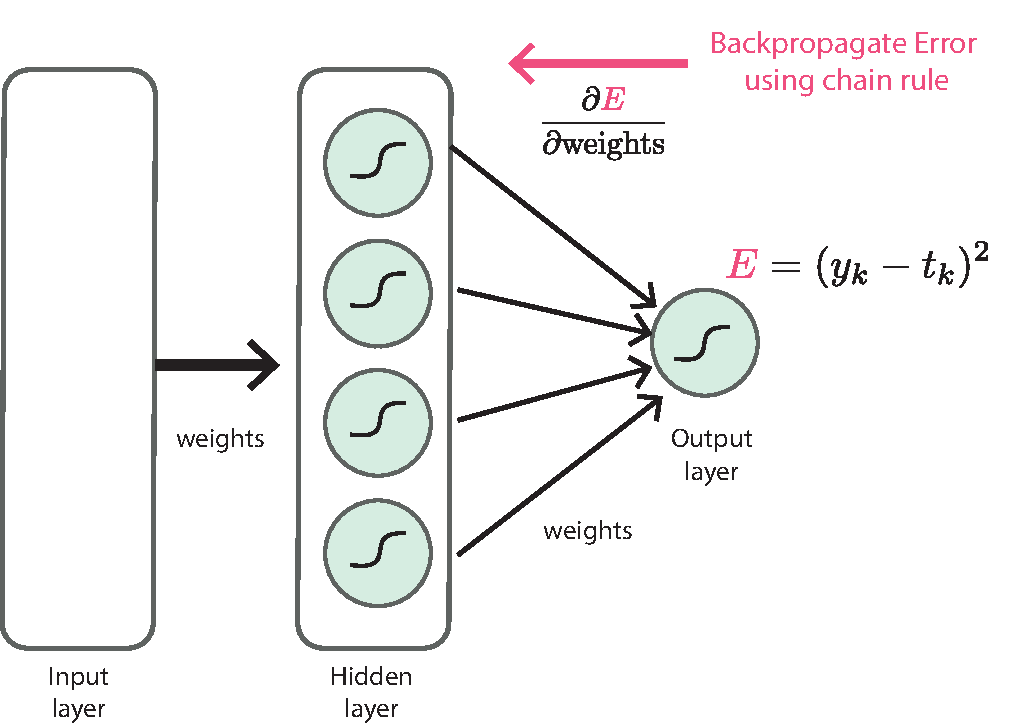
\includegraphics[scale=0.5]{figures/MLP_back.pdf}}

\small This is a special case where the output layer has a single
node. In the general case we could have e.g.\ $E = \sum_{k} (y_{k}-t_{k})^{2}$.

\end{frame}


% \begin{frame}[fragile]
% \frametitle{Neural networks -- backward pass}

% \small We now need to optimise our weights, and as before we use derivatives to find a solution. Effectively backpropagating the output error signal across the network -- backpropagation algorithm.

% \begin{enumerate}
% 	\item \small Compute the error (or cost) function: e.g.: $E = \mathlarger{\frac{1}{2}\sum_{n=1}^N} (\bm{y(x_n,w}) - \bm{t_n})^2$
% \uncover<2->{	\item \small Use the \emph{chain rule} to compute the gradients w.r.t. $\bm{w}$, $\frac{dE}{d\bm{w}}$
% 	\item \small For the output weights $w_{kj}$ we get:\\ $\mathlarger{\frac{\partial E}{\partial w_{kj}} = \frac{\partial E}{\partial y_{k}} \frac{\partial y_k}{\partial a_k} \frac{\partial a_k}{\partial w_{kj}} = \sigma'(y_n - t_n)z_j}$ \footnote{$\sigma '$ denotes the derivative of the sigmoid activation function.}}
% \uncover<3->{	\item \small Whereas for the input weights $w_{ji}$ we get: \\$\mathlarger{\frac{\partial E}{\partial w_{ji}} = \frac{\partial E}{\partial y_{k}} \frac{\partial y_k}{\partial a_k} \frac{\partial a_k}{\partial z_{j}}  \frac{\partial z_j}{\partial a_j} \frac{\partial a_j}{\partial w_{ji}} = \sigma' (y_n - t_n) w_{kj}^T \sigma' x_i}$ \footnote{Note that the updates for the bias terms $w_0$ do not depend on the activity of the previous layer $z_j$ and $x_i$.}}
% \end{enumerate}

% \end{frame}
%%%%%%%%%%%%%%%%%%%%%%%%%%%%%%%%%%%%%%%%%%%%%%%%%%%%%%%%%%%%%%%%%%%%%%
\begin{titledslide}{Total error as a sum of datapoint errors}

  \begin{itemize}
  \item Typically the error for an entire dataset breaks down into a
    sum of errors for each individual datapoint:
  \end{itemize}
  \[
    E(\mathbf{w}) = \sum_{n=1}^{N}E_{n}(\mathbf{w})
  \]
  \begin{itemize}
  \item This means that the error gradient for the entire dataset with
    respect to some weight $w_{ji}$ will just be the sum of error
    gradients for each datapoint: 
  \end{itemize}
  \[
    \frac{\partial E}{\partial w_{ji}} = \sum_{n=1}^{N}\frac{\partial E_{n}}{\partial w_{ji}}
  \]
  \begin{itemize}
  \item So we focus attention on computing the $\frac{\partial
      E_{n}}{\partial w_{ji}}$ values.
  \end{itemize}
\end{titledslide}
%%%%%%%%%%%%%%%%%%%%%%%%%%%%%%%%%%%%%%%%%%%%%%%%%%%%%%%%%%%%%%%%%%%%%%
\begin{titledslide}{Computing partial derivatives 1}

  \begin{itemize}
  \item Although all values in the network depend on the datapoint $n$
    we're focusing on, we will (like Bishop) omit the subscript $n$ from network
    values to reduce clutter.
  \item Consider an arbitrary unit $j$ (aka `node') in an neural
    network.
  \item We will associate the \emph{bias} for a unit with a dummy
    input fixed to 1.
  \item The unit computes a value $z_j$ by first computing $a_j$, a weighted sum of its
    inputs (from the previous layer), and then sending $a_j$ to some nonlinear
    \emph{activation function} $h$:
  \end{itemize}
  \begin{align}
    \label{eq:preact}
    a_{j} & = \sum_{i}w_{ji}z_{i} \\
    \label{eq:act}
    z_{j} & = h(a_{j}) \\
  \end{align}
  \begin{itemize}
  \item Since $E_n$ (the error for the $n$th datapoint) only depends on
    weight $w_{ji}$ via $a_{j}$ we can use the chain rule to write:
  \end{itemize}
  \[
    \frac{\partial E_{n}}{\partial w_{ji}} =     \frac{\partial E_{n}}{\partial a_{j}}\frac{\partial a_{j}}{\partial w_{ji}}
  \]
  
\end{titledslide}
%%%%%%%%%%%%%%%%%%%%%%%%%%%%%%%%%%%%%%%%%%%%%%%%%%%%%%%%%%%%%%%%%%%%%%
\begin{titledslide}{Computing partial derivatives 2}

  \[
    \frac{\partial E_{n}}{\partial w_{ji}} =     \frac{\partial E_{n}}{\partial a_{j}}\frac{\partial a_{j}}{\partial w_{ji}}
  \]
  \begin{itemize}
  \item Since  $a_{j}  = \sum_{i}w_{ji}z_{i} $, $\frac{\partial a_{j}}{\partial w_{ji}}$ is easy to compute:
  \end{itemize}
  \[
    \frac{\partial a_{j}}{\partial w_{ji}} = z_{i}
  \]
  As for $\frac{\partial E_{n}}{\partial a_{j}}$ let's just introduce
  some notation for now: $\delta_{j} \equiv \frac{\partial E_{n}}{\partial a_{j}}$
  \begin{equation}
    \label{eq:dz}
    \frac{\partial E_{n}}{\partial w_{ji}} = \delta_{j}z_{i}
  \end{equation}

\end{titledslide}
%%%%%%%%%%%%%%%%%%%%%%%%%%%%%%%%%%%%%%%%%%%%%%%%%%%%%%%%%%%%%%%%%%%%%%
\begin{titledslide}{Computing partial derivatives 3}

  \begin{itemize}
  \item We compute the $\delta_{j} \equiv \frac{\partial
      E_{n}}{\partial a_{j}}$ \emph{backwards}, starting with the
    output units.
  \item For example, if the error (for a single datapoint) is $E_{n} =
    \frac{1}{2}\sum_{k} (y_{k}-t_{k})^{2}$ where $y_k=h(a_k)$ then:
  \end{itemize}
  \begin{equation}
    \label{eq:outgrad}
    % \delta_{k} = y_{k}-t_{k}    
\delta_k \equiv 
\frac{\partial E_n}{\partial a_k}
=
\frac{\partial E_n}{\partial y_k}
\frac{\partial y_k}{\partial a_k}
=
\bigl(y_k - t_k\bigr)\, h'(a_k)
  \end{equation}
  \begin{itemize}
  \item For the hidden units we use (a multivariable version of) the chain rule:
  \end{itemize}
  \[
    \delta_{j} \equiv \frac{\partial E_{n}}{\partial a_{j}} = \sum_{k} \frac{\partial E_{n}}{\partial a_{k}}\frac{\partial a_{k}}{\partial a_{j}} 
  \]
  ``where the sum runs over all units $k$ to which unit $j$ sends
  connections'' (Bishop). ``we are
making use of the fact that variations in $a_j$ give rise to
variations in the error function only through variations in the
variables $a_k$.'' (Bishop).
\end{titledslide}
%%%%%%%%%%%%%%%%%%%%%%%%%%%%%%%%%%%%%%%%%%%%%%%%%%%%%%%%%%%%%%%%%%%%%%
\begin{titledslide}{Computing partial derivatives 4}

  \[
    \delta_{j} \equiv \frac{\partial E_{n}}{\partial a_{j}} = \sum_{k} \frac{\partial E_{n}}{\partial a_{k}}\frac{\partial a_{k}}{\partial a_{j}} 
  \]
  can be reformulated to give the \emph{backpropagation formula}:
  \begin{equation}
    \label{eq:backprop}
    \delta_{j} = h'(a_{j})\sum_{k}w_{kj}\delta_{k}
  \end{equation}
    
\end{titledslide}
%%%%%%%%%%%%%%%%%%%%%%%%%%%%%%%%%%%%%%%%%%%%%%%%%%%%%%%%%%%%%%%%%%%%%% 
\begin{titledslide}{Error Backpropagation}

  As given in Bishop:

  \begin{enumerate}
  \item Apply an input vector $\mathbf{x}_n$ to the network and
    forward propagate through the network using (\ref{eq:preact}) and
    (\ref{eq:act}) to find the activations of all the hidden and
    output units.
  \item Evaluate the $\delta_k$ for all the outputs units using
    e.g.\ (\ref{eq:outgrad}).
   \item Backpropagate the $\delta$'s using (\ref{eq:backprop}) to
     obtain $\delta_j$ for each hidden unit in the network.
  \item Use (\ref{eq:dz}) to evaluate the required derivatives.
  \end{enumerate}

  \vspace*{1cm}
  
  \begin{itemize}
  \item A key point is that computing a $\delta_j$ value helps us
    compute \textbf{several} other $\delta_{j'}$ values.
  \end{itemize}
  
\end{titledslide}
%%%%%%%%%%%%%%%%%%%%%%%%%%%%%%%%%%%%%%%%%%%%%%%%%%%%%%%%%%%%%%%%%%%%%%
\begin{titledslide}{Backpropagation in practice}

  \begin{itemize}
  \item It is crucial to organise the computation of all these partial
    derivatives (i.e.\ the gradient $\partial E / \partial
    \mathbf{w}$) efficiently.
  \item The quantities required will be organised in tensors
    (generalisation of matrices beyond 2 dimensions).
  \item The \texttt{PyTorch} approach is called \emph{Autograd}.
    There's lots of useful info/explanation of how it works on the
    PyTorch site.
  \end{itemize}

\includegraphics[scale=0.1]{figures/Pytorch_logo.png}
  \begin{quotation}
    PyTorch's Autograd feature is part of what make PyTorch flexible
    and fast for building machine learning projects. It allows for the
    rapid and easy computation of multiple partial derivatives (also
    referred to as gradients) over a complex computation. This
    operation is central to backpropagation-based neural network
    learning. \href{https://pytorch.org/tutorials/beginner/introyt/autogradyt\_tutorial.html}{The
    Fundamentals of Autograd}
  \end{quotation}


\end{titledslide}

%%%%%%%%%%%%%%%%%%%%%%%%%%%%%%%%%%%%%%%%%%%%%%%%%%%%%%%%%%%%%%%%%%%%%% 
\begin{frame}[fragile]
\frametitle{Neural networks -- gradient descent \footnote{\tiny Its called descent because we are minimising the cost function, so descending on the function landscape, which can be quite hilly!}}

\small In many ML methods it is common to iteratively update the parameters by descending the gradient. \vspace{10pt}\\

\centerline{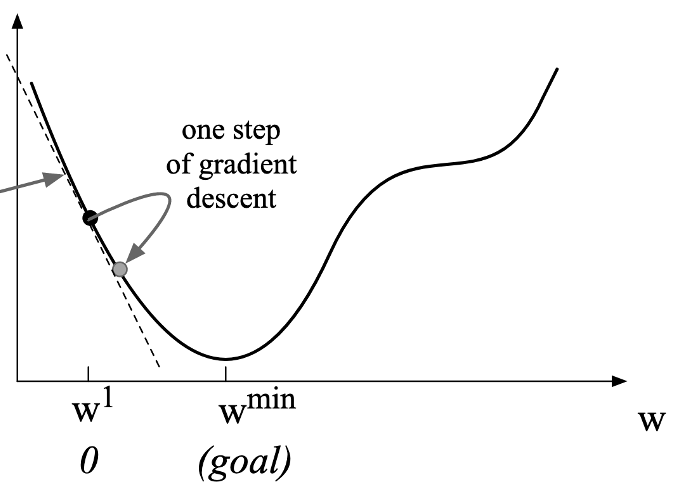
\includegraphics[scale=0.25]{figures/gradient_descent.png}\footnote{\tiny
    Figure from
    \url{https://mc.ai/an-introduction-to-gradient-descent-2/} (link
    no longer working)}}

\uncover<2->{In our neural network this means to update the weights using:

\begin{itemize}
	\item \small $w_{ji}^{new} = w_{ji}^{old} - \Delta w_{ji}$, where $\Delta w_{ji} = \sigma'(a_{k}) (y_n - t_n) w_{kj} \sigma'(a_{j}) x_i$
	\item \small $w_{kj}^{new} = w_{kj}^{old} - \Delta w_{kj}$, where $\Delta w_{kj} = \sigma'(a_{k})(y_n - t_n)z_j$
    \item \small
$w_{kj}^{new} = w_{kj}^{old} - {\color{red}\eta}\,\Delta w_{kj}$,
where $\eta$ denotes the learning rate.

	\item \small This is often done in mini-batches -- using a small number of samples to compute $\Delta w$.
\end{itemize}}

\end{frame}




\begin{frame}[fragile]
\frametitle{Neural networks}

\begin{example}
Using sklearn we fitted a MLP classifier to the data: \vspace{5pt}\\	
\centerline{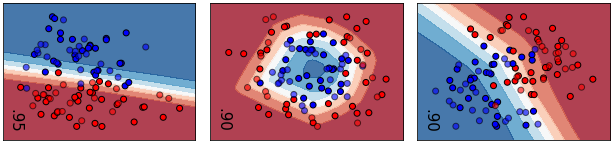
\includegraphics[scale=0.5]{figures/nnet_class.png}}
\end{example}
\small An MLP with one hidden layer can perform well in nonlinear classification problems. 

However, because MLPs are highly flexible  they can easily \emph{overfit}. 

Solutions: \emph{early stopping} (stop when test performance starts decreasing) and \emph{regularisation} methods such as \emph{dropout} (randomly turn off units during training).
\end{frame}




\begin{frame}[fragile]
\frametitle{Classification methods -- overall comparison}

\centerline{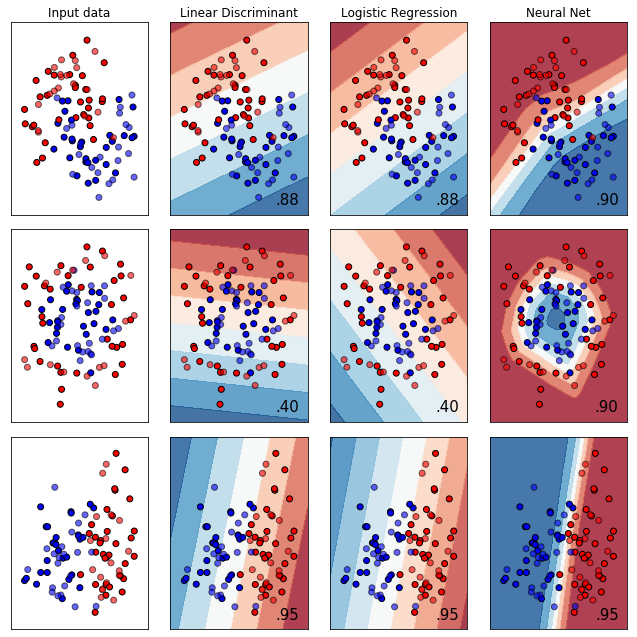
\includegraphics[scale=0.35]{figures/classifiers_comparison_this.png}}

\end{frame}



\begin{frame}[fragile]
\frametitle{Classification methods -- overall comparison \small [we
  don't cover all these methods]}

\centerline{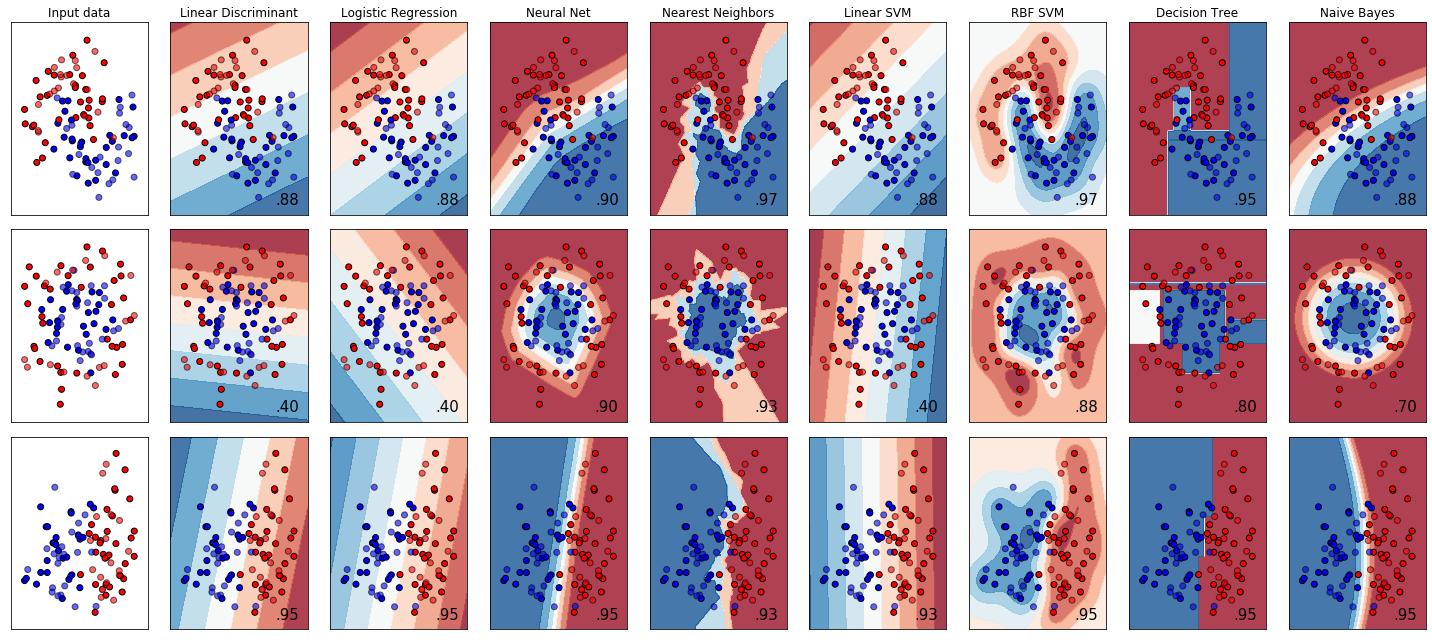
\includegraphics[scale=0.25]{figures/classifiers_comparison.png}}
\end{frame}
%%%%%%%%%%%%%%%%%%%%%%%%%%%%%%%%%%%%%%%%%%%%%%%%%%%%%%%%%%%%%%%%%%%%%%
\begin{titledslide}{Reading}

  \begin{itemize}
  \item Bishop \S5.1 except \S5.1.1
  \item Bishop \S5.2 except \S5.2.2
  \item Bishop \S5.3 up to \S5.3.2
  \item Murphy \S13.1-\S13.2
  \item Murphy's description of backpropagation in \S13.3 is
    interesting since it is closer to how it is actually implemented,
    but more complex than Bishop's presentation.
  \end{itemize}
  \vspace{1em}
  \centering
  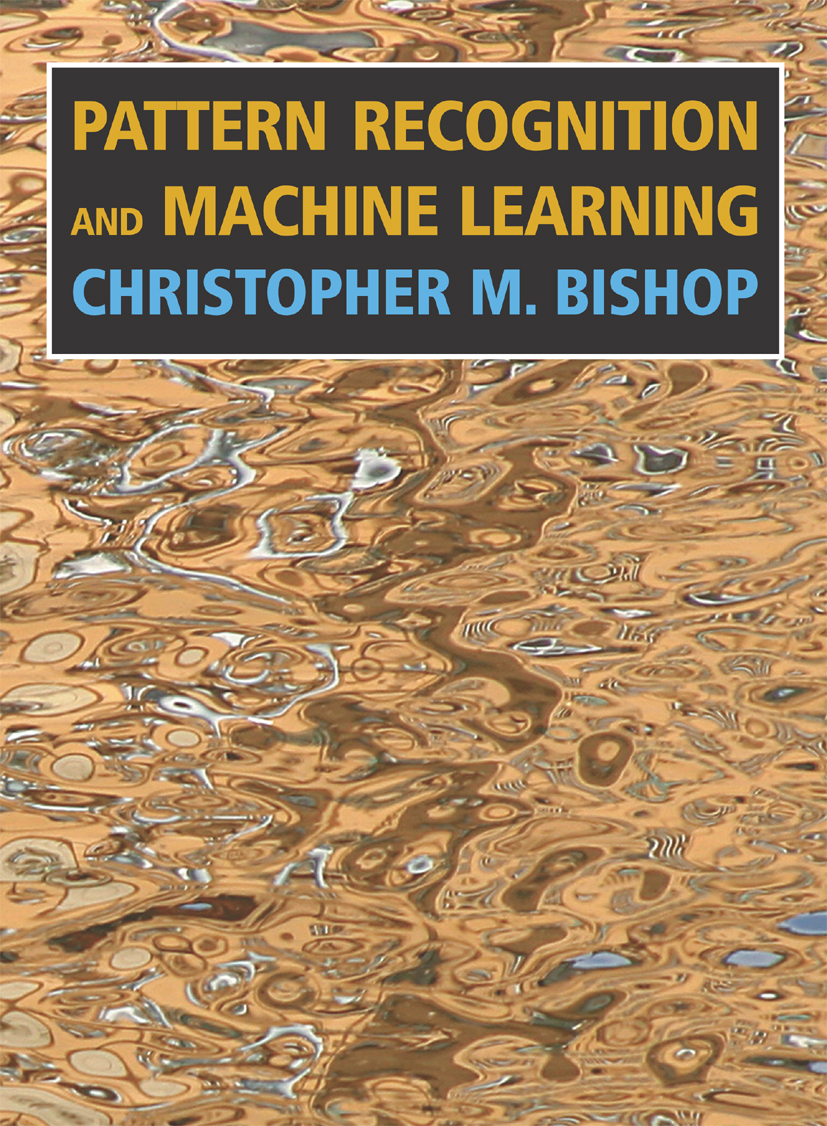
\includegraphics[height=3cm]{figures/bishop.jpg}\hspace{4 em}%
  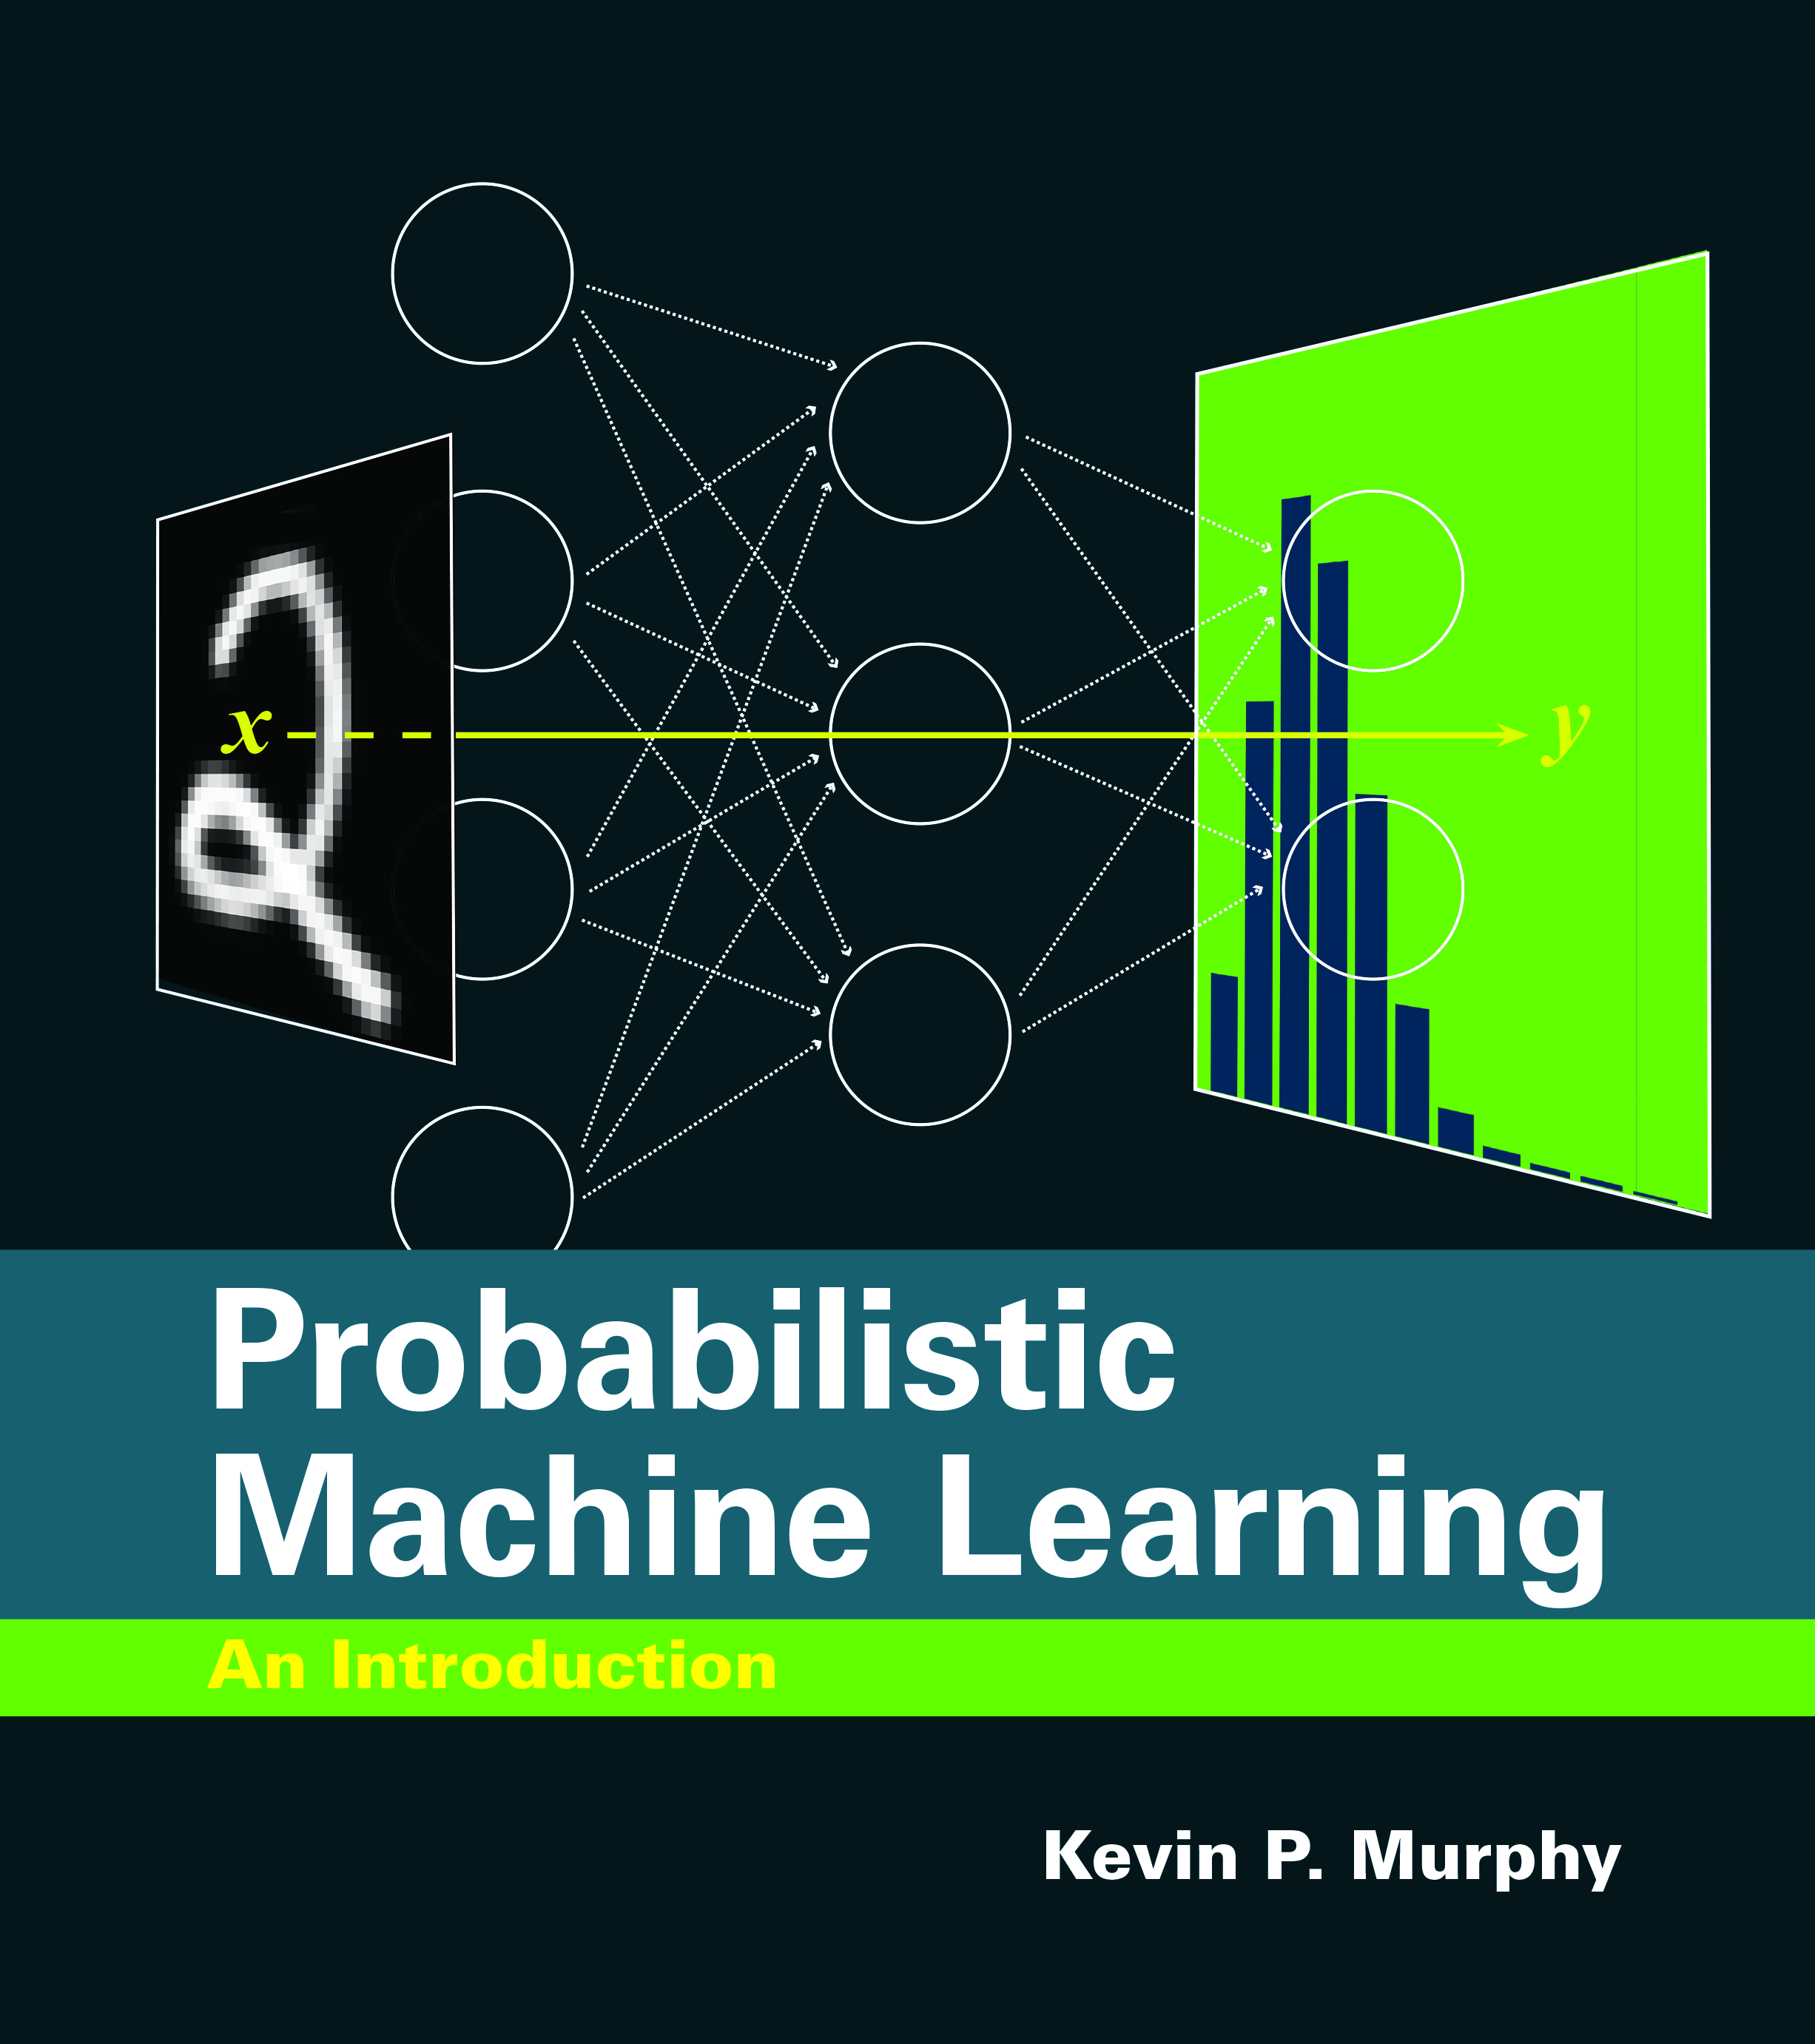
\includegraphics[height=3cm]{figures/murphy.jpg}
  
\end{titledslide}
%%%%%%%%%%%%%%%%%%%%%%%%%%%%%%%%%%%%%%%%%%%%%%%%%%%%%%%%%%%%%%%%%%%%%%
\begin{titledslide}{Exercises and lab/practical}

  \begin{itemize}
  \item Bishop Exercise 4.12
  \item Bishop Exercise 5.6 (Tip: Use the result you derived in
    Exercise 4.12 to help you.) 
  \item Lab/Practical:
    \begin{itemize}
    \item Week~2: Neural Networks
    \end{itemize}
  \end{itemize}
  
\end{titledslide}
%%%%%%%%%%%%%%%%%%%%%%%%%%%%%%%%%%%%%%%%%%%%%%%%%%%%%%%%%%%%%%%%%%%%%%
\end{document}

